\section{Detecting Similar Languages} \label{sec:cluster}

To exemplify the use of SeedLing for computational research on low-resource languages, we experiment with automatic detection of similar languages. When working on endangered languages, documentary and computational linguists alike face a lack of resources. It is often helpful to exploit lexical, syntactic or morphological knowledge of related languages. For example, similar high-resource languages can be used in bootstrapping approaches, such as described by \newcite{yarowsky:ngai:2001} or \newcite{xia2007multilingual}.

Language classification can be carried out in various ways. Two common approaches are genealogical classification, mapping languages onto family trees according to their historical relatedness \cite{swadesh1952,starostin2010}; and typological classification, grouping languages according to linguistic features \cite{georgi2010wals,daume2009}. Both of these approaches require linguistic analysis. By contrast, we use surface features (character n-gram and word unigram frequencies) extracted from SeedLing, and apply an off-the-shelf hierarchical clustering algorithm.\footnote{\url{http://www.scipy.org}} Specifically, each language is represented as a vector of frequencies of character bigrams, character trigrams, and word unigrams. Each of these three components is normalised to unit length.  Data was taken from ODIN, Omniglot, and the UDHR.

\paragraph{Experimental Setup.}
We first perform hierarchical clustering, which produces a tree structure: each leaf represents a language, and each node a cluster. We use linkage methods, which recursively build the tree starting from the leaves. Initially, each language is in a separate cluster, then we iteratively find the closest two clusters and merge them. Each time we do this, we take the two corresponding subtrees, and introduce a new node to join them.

We define the distance between two clusters by considering all possible pairs of languages, with one from each cluster, and taking the largest distance. We experimented with other ways to define the distance between clusters, but results were poor and we omit results for brevity.

To ease evaluation, we produce a partitional clustering, by stopping when we reach a certain number of clusters, set in advance.

\begin{table}[t]
\centering
    \begin{tabular}{l|ccc}
    ~        & Precision & Recall       & F-score \\ \hline
	SeedLing	& 0.255	& 0.205	& 0.150 \\ \hline
	Base. 1: random	& 0.184	& 0.092	& 0.068 \\
	Base. 2: together	& 0.061	& 1.000	& 0.112 \\
	Base. 3: separate	& 1.000	& 0.086	& 0.122
    \end{tabular}
\caption{Clustering compared with baselines}
\label{table:cluster}
\end{table}

\begin{figure}[t]
\begin{centering}
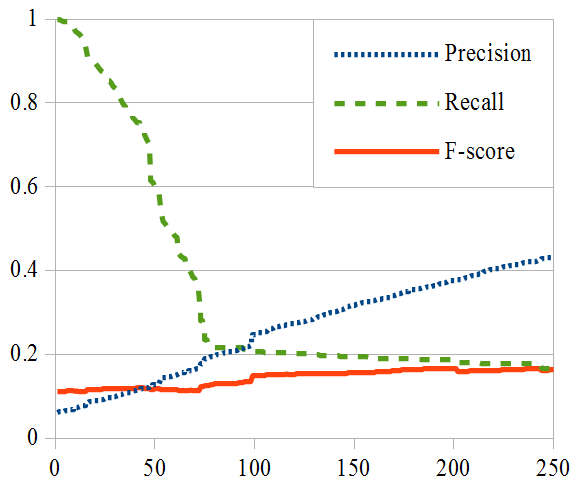
\includegraphics[scale=0.75]{performance.png}
\caption{Performance against number of clusters}
\label{fig:performance}
\end{centering}
\end{figure}

\paragraph{Evaluation.}
We compare our clustering to the language families in Ethnologue. However, there are many ways to evaluate clustering quality. \newcite{amigo2009metrics} propose a set of criteria which a clustering evaluation metric should satisfy, and demonstrate that most popular metrics fail to satisfy at least one of these criteria.  However, they prove that all criteria are satisfied by the BCubed metric, which we therefore adopt.  To calculate the BCubed score, we take the induced cluster and gold standard class for each language, and calculate the F-score of the cluster compared to the class.  These F-scores are then averaged across all languages.

In Table \ref{table:cluster}, we set the number of clusters to be 105, the number of language families in our data, and compare this with three baselines: a random baseline (averaged over 20 runs); putting all languages in a single cluster; and putting each language in a separate cluster. Our clustering outperforms all baselines. It is worth noting that precision is higher than recall, which is perhaps expected, given that related languages using wildly differing orthographies will appear distinct.

To allow a closer comparison with \newcite{georgi2010wals}, we calculate pairwise scores - i.e. considering if pairs of languages are in the same cluster or the same class. For 105 clusters, we achieve a pairwise f-score of 0.147, while Georgi et al. report 0.140. The figures are not quite comparable since we are evaluating over a different set of languages; nonetheless, we only use surface features, while Georgi et al. use typological features from WALS.  This suggests the possibility for cross-linguistic research to be conducted based on shallow features.

In Figure \ref{fig:performance}, we vary the number of clusters. The highest f-score is obtained for 199 clusters. There is a notable jump in performance between 98 and 99, just before the true number of families, 105.

Interpreting the clusters directly is difficult, because they are noisy.  However, the distribution of cluster sizes mirrors the true distribution - for 105 clusters, we have 48 clusters of size 1 or 2, with the largest cluster of size 130; while in our gold standard, there are 51 families with only 1 or 2 languages in the data, with the largest of size 150.
